\documentclass{article}
\pdfoutput=1
\usepackage[utf8]{inputenc}
\usepackage[T1]{fontenc}
\usepackage{microtype, natbib}
\usepackage{amsmath,amssymb,amsthm,enumerate,tikz}
\PassOptionsToPackage{hyphens}{url}\usepackage{hyperref}
\usepackage{xcolor}
%% \usepackage{bussproofs,xcolor,stackengine}
\hypersetup{
  colorlinks,
  linkcolor={red!70!black},
  citecolor={green!50!black},
  urlcolor={blue!50!black}
}

\newcommand{\fa}[2]{\ensuremath{\Pi(#1),\ #2}}
\newcommand{\fax}[2]{\ensuremath{\Pi#1,\ #2}}
\newcommand{\ex}[2]{\ensuremath{\Sigma(#1),\ #2}}
\newcommand{\empt}{\ensuremath{\mathbf{0}}}
\newcommand{\unit}{\ensuremath{\mathbf{1}}}
\newcommand{\bool}{\ensuremath{\mathbf{2}}}
\DeclareMathOperator{\myap}{ap}
\DeclareMathOperator{\myapd}{apd}
\DeclareMathOperator{\colim}{colim}

\DeclareMathOperator{\homm}{hom}
\DeclareMathOperator{\Id}{Id}
\DeclareMathOperator{\ind}{ind}
\DeclareMathOperator{\transport}{transport}
\DeclareMathOperator{\quotient}{quotient}
\newcommand{\Kloop}{K\textnormal{-loop}}
\newcommand{\Kelim}{K\textnormal{-elim}}
\newcommand{\id}{\textnormal{id}}
\newcommand{\istrunc}[1]{\textnormal{is-}#1\textnormal{-type}}
\newcommand{\refl}{\textnormal{refl}}
\newcommand{\base}{\textnormal{base}}
\newcommand{\lp}{\textnormal{loop}}
\newcommand{\surf}{\textnormal{surf}}
\newcommand{\isprop}{\textnormal{is-prop}}
\newcommand{\isset}{\textnormal{is-set}}
\newcommand{\prop}{\textnormal{Prop}}
%% \newcommand{\tr}{\textnormal{tr}}
\newcommand{\ap}[2]{\ensuremath{\myap_{#1}(#2)}}
\newcommand{\apd}[2]{\ensuremath{\myapd_{#1}(#2)}}
\newcommand{\eps}{\ensuremath{\varepsilon}}
\newcommand{\N}{\mathbb{N}}
\newcommand{\U}{\mathcal{U}}
\newcommand{\sph}{\mathbb{S}}
\newcommand{\sy}{\ensuremath{^{-1}}}
\newcommand{\myurl}[1]{\href{#1}{\path{#1}}}

%% Theorem environment declarations (using amsthm):
\newtheorem{theorem}{Theorem}[section]
\newtheorem{axiom}[theorem]{Axiom}
\newtheorem{fact}[theorem]{Fact}
\newtheorem{proposition}[theorem]{Proposition}
\newtheorem{lemma}[theorem]{Lemma}
\newtheorem{corollary}[theorem]{Corollary}

\theoremstyle{definition}
\newtheorem{definition}[theorem]{Definition}
\newtheorem{convention}[theorem]{Convention}
\newtheorem{example}[theorem]{Example}
\newtheorem{examples}[theorem]{Examples}
\newtheorem{notation}[theorem]{Notation}
\theoremstyle{remark}
\newtheorem{remark}[theorem]{Remark}
\newtheorem{idea}[theorem]{Idea}
\usetikzlibrary{arrows}
\usetikzlibrary{calc}

\renewcommand{\epsilon}{\varepsilon}
\renewcommand{\theta}{\vartheta}
\renewcommand{\kappa}{\varkappa}
\renewcommand{\rho}{\varrho} % remember my teacher and friend Adalberto!
\renewcommand{\phi}{\varphi}

\begin{document}

\title{Notes on Eilenberg-Maclane Spaces}

\author{Floris van Doorn}
\maketitle

\begin{abstract}
In homotopy type theory, we prove the categorical properties of Eilenberg-Maclane spaces. The proofs
are fully formalized in Lean. We prove that the category of $n$-connected $(n+1)$-truncated pointed
types is equivalent to the category of groups for $n = 0$ and the category of abelian groups for $n
\geq 1$.
\end{abstract}

\section{Preliminaries}
\begin{definition}
\mbox{}
\begin{itemize}
  \item A \emph{pointed type} is a type $X$ together with a specified basepoint $x_0 : X$. We
    usually write $X$ for $(X,x_0)$.
  \item A \emph{pointed map} between pointed types $X$ and $Y$ is a map $f : X \to Y$ together with
    a proof that $f$ respects the basepoint, i.e. a path $f_0 : f(x_0) = y_0$. We usually write $f$
    for $(f,f_0)$.
  \item A pointed homotopy between pointed maps $f, g : X \to Y$ is a homotopy $h : f ~ g$ together
    with the proof that the homotopy respects the specified paths, i.e. $h_0 : h(x_0) \cdot g_0 =
    f_0$. We write $h$ for $(h,h_0)$.
  \item A pointed equivalence $f : X \simeq Y$ is a pointed map where the underlying map is an
    equivalence. Note that the notation $\simeq$ can mean three things: equivalence of types,
    pointed equivalence or group isomorphism. It should always be interpreted as the notion which
    preserves as much structure as the type exhibit, unless specified otherwise.
  \item The \emph{suspension} of a type $X$ is the higher inductive type generated by two points,
    north and south, and a meridian for every point in $X$. In a scheme: \\
    \texttt{HIT} $\Sigma X :=$ \\
    $\bullet\ N : \Sigma X$; \\
    $\bullet\ S : \Sigma X$; \\
    $\bullet\ merid : X \to N = S$. \\
    The suspension is a pointed type by taking $N$ as its basepoint.
  \item For $n\geq -2$, the $n$-truncation of a type $X$ is the type $X$ where all path structure
    above level $n+1$ is removed. \\
    \texttt{HIT} $\|X\|_n :=$ \\
    $\bullet\ |{-}|_n : X \to \|X\|_n$; \\
    $\bullet\ \eps : \istrunc{n}(\|X\|_n)$. \\
    Alternatively, if one doesn't accept a ``path constructor'' like $\eps$, one can define the $n$-truncation using more conventional point and path constructors as using hubs and a spokes:
    \texttt{HIT} $\|X\|_n :=$ \\
    $\bullet\ |{-}|_n : X \to \|X\|_n$; \\
    $\bullet\ h : (\sph^{n+1}\to\|X\|_n)\to\|X\|_n$; \\
    $\bullet\ s : \fax{(r : \sph^{n+1}\to\|X\|_n)(x : \sph^{n+1})}{r(x)=h(r)}$. \\
    If $X$ is a pointed type, then $\|X\|_n$ is pointed with basepoint $|x_0|_n$.
    \item Both the suspension and the $n$-truncation act functorially. If $f : X \to Y$ is a pointed
      map, then there are pointed maps $\|f\|_n : \|X\|_n \to \|Y\|_n$ and $\Sigma f : \Sigma X \to
      \Sigma Y$.
    \item $\Sigma \dashv \Omega$.
    \item If $G$ is a (pre-)groupoid, the groupoid quotient is a higher inductive type with
      constructors\\
    \texttt{HIT} $\quotient(G) :=$ \\
    $\bullet\ i : G_0 \to \quotient(G)$; \\
    $\bullet\ p : \fa{x\ y : G_0}{\homm(x,y)\to x=y}$; \\
    $\bullet\ q : \fax{(x\ y\ z : G_0)(g : \homm(y,z))(f : \homm(x,y))}
           {p(g \circ f) = p(f) \cdot p(g)}$. \\
    $\bullet\ \eps : \istrunc{1}(\quotient(G))$. \\
    As with the $n$-truncation, the fact that the groupoid quotient is 1-truncated can be encoded
    using hubs and spokes.
\end{itemize}
\end{definition}

\begin{lemma}
The following results will be used below.
\begin{itemize}
\item $\Omega^k\|X\|_{n+k}\simeq \|\Omega^k X\|_n$ (as pointed types).
\item If $X \simeq Y$ as pointed types then $\pi_n(X) \simeq \pi_n(Y)$.
\item $\pi_k(\Omega^n X)\simeq \pi_{n+k}(X)$.
\end{itemize}
\end{lemma}
\section{Eilenberg-Maclane Spaces}
In \cite{Licata2014EM} the authors define Eilenberg-Maclane spaces. We use the same approach as in
that paper. We quickly review the results in that paper.

\subsection{Review}

If $G$ is any group, the 1-dimensional Eilenberg-Maclane space $K(G,1)$ can be defined by viewing
$G$ as a groupoid, and taking the groupoid quotient of $G$. It is not hard to see that $G$ is
0-connected and 1-truncated. Using an encode-decode proof, one shows $\Omega K(G,1) \simeq G$ and
that this equivalence seconds concatenation to multiplication. Hence the composite
$\pi_1K(G,1)\simeq \|G\|_0\simeq G$ is a group isomorphism.

If $G$ is Abelian, the higher Eilenberg-Maclane spaces can be defined recursively
as $$K(G,n+1):\equiv \|\Sigma K(G,n)\|_{n+1}$$ for $n\geq 1$. This definition is slightly different
than the one given in \cite{Licata2014EM}, where $K(G,n+1)$ was defined using the iterated
suspension as $\|\Sigma^n K(G,1)\|_{n+1}$. We chose to modify the definition, since a lot of
properties of Eilenberg-Maclane spaces are proven by induction on $n$, so it is more convenient to
have $K(G,n+1)$ defined directly in terms of $K(G,n)$.

It's not hard to show that $K(G,n)$ is $(n-1)$-connected and $n$-truncated. Trickier is to show that
$\Omega K(G,n+1)\simeq K(G,n)$. This is done separately for $n=1$ and for $n\geq 2$.

For $n=1$ we need the result that for every type $X$ with a coherent h-structure, the type $\|\Sigma
X\|_2$ is a \emph{delooping} of $X$, which means that $\Omega \|\Sigma X\|_2 \simeq X$. If $G$ is abelian, then $K(G,1)$ can be equipped with a coherent h-structure,
showing that $\Omega K(G,2)\simeq K(G,1)$.

For $n\geq 2$, this can be done using the Freudenthal Suspension Theorem, which states that if $X$
is $n$-connected and $k\leq 2n$, then $\|\Omega\Sigma X\|_k\simeq \|X\|_k$. Then the equivalence
follows from the following chain:
$$\Omega K(G,n+1)\equiv \Omega\|\Sigma K(G,n)\|_{n+1}\simeq \|\Omega\Sigma K(G,n)\|_n\simeq
\|K(G,n)\|_n\simeq K(G,n).$$ The Freudenthal Suspension Theorem is applied in the third step, which
is allowed since $K(G,n)$ is $(n-1)$-connected and $n \leq 2(n-1)$ for $n\geq2$.

This finishes the proof sketch that $\Kloop(G,n):\Omega K(G,n+1)\simeq K(G,n)$. By induction,
$\Omega^n K(G,n+1)\simeq K(G,1)$, hence we get the following isomorphism of groups
$\pi_{n+1}(K(G,n+1))\simeq \pi_1(K(G,1))\simeq G$.

\subsection{Uniqueness}

In this section we prove that Eilenberg-Maclane spaces are unique, which means that if $X$ and $Y$
are both $(n-1)$-connected, $n$-truncated pointed types such that $\pi_n(X)\simeq \pi_n(Y)$, then
$X\simeq Y$. Note that from these assumptions one can show that $\pi_k(X)\simeq 1\simeq \pi_k(Y)$
for $k < n$ since $X$ and $Y$ are $(n-1)$-connected, but also for $k > n$ since $X$ and $Y$ are
$n$-truncated. Hence from the assumptions we actually have that $\pi_k(X)\simeq\pi_k(Y)$ for all
natural numbers $k$.

This is similar to Whitehead's Theorem, which states that if $f : X \to Y$ is a pointed map
which induces an equivalence on all homotopy groups, then $f$ is an equivalence. Whitehead's Theorem
is not true in general, but it is true under the assumption that both $X$ and $Y$ are $n$-truncated
for some $n$. For the special case that $X$ and $Y$ are both $(n-1)$-connected and $n$-truncated one
doesn't need to find a map between $X$ and $Y$ to show that they are equivalent, as long as they
have isomorphic homotopy groups.

We first give an elimination principle for $K(G,n)$.
\begin{definition}
Suppose that $X$ is an $(n-1)$-connected $n$-truncated pointed type, and suppose that for some group
$G$ there is an equivalence $e : \Omega^n X \simeq G$ which sends concatenation to
multiplication. Then there is a pointed map $\Kelim(e, n) : K(G,n)\to X$.
\end{definition}
\begin{proof}[Construction]
  We construct this by induction on $n$.
\end{proof}

\begin{lemma}
There is a pointed homotopy making the following diagram commute.
\begin{center}
  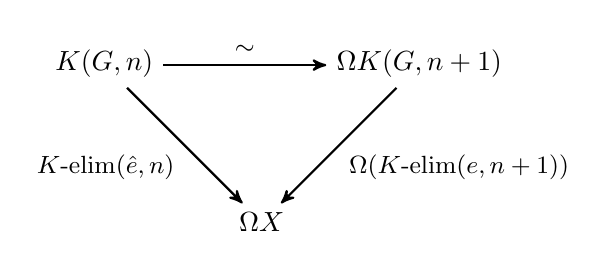
\begin{tikzpicture}[>=stealth',auto,node distance=3cm,
      thick,main node/.style={font=\sffamily\bfseries},text height=1.5ex]
    \node[main node] (Kn) at (0,0) {$K(G,n)$};
    \node[main node] (OK) at (4,0) {$\Omega K(G,n+1)$};
    \node[main node] (OX) at (2,-2) {$\Omega X$};
         \path[every node/.style={font=\sffamily\small}]
         (Kn) edge [->] node {$\sim$} (OK)
              edge [->] node [below left] {$\Kelim(\hat e,n)$} (OX)
         (OK) edge [->] node [below right] {$\Omega(\Kelim(e,n+1))$} (OX);
  \end{tikzpicture}
\end{center}

\end{lemma}
\begin{proof}
\end{proof}

\begin{lemma}
The following diagram commutes.%TODO: this can be done easier in formalization.
\begin{center}
  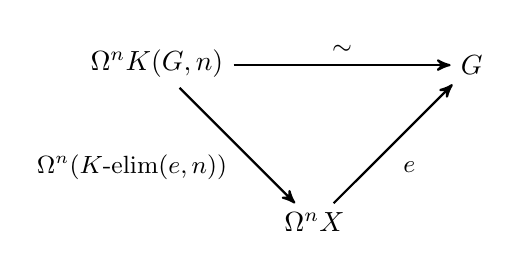
\begin{tikzpicture}[>=stealth',auto,node distance=3cm,
      thick,main node/.style={font=\sffamily\bfseries},text height=1.5ex]
    \node[main node] (OK) at (0,0) {$\Omega^nK(G,n)$};
    \node[main node] (G)  at (4,0) {$G$};
    \node[main node] (OX) at (2,-2) {$\Omega^n X$};
         \path[every node/.style={font=\sffamily\small}]
         (OK) edge [->] node {$\sim$} (G)
              edge [->] node [below left] {$\Omega^n(\Kelim(e,n))$} (OX)
         (OX) edge [->] node [below right] {$e$} (G);
  \end{tikzpicture}
\end{center}

\end{lemma}
\begin{proof}
\end{proof}

\begin{theorem}
$\Kelim(e,n)$ is an equivalence.
\end{theorem}
\begin{proof}
\end{proof}

\begin{corollary}
The type of $(n-1)$-connected, $n$-truncated pointed types is equivalent to the type of groups for
$n=1$ and equivalent to the type of Abelian groups for $n \geq 2$.
\end{corollary}
\begin{proof}
\end{proof}

\subsection{Categories}
\begin{definition}
  If $\phi : G \to H$ is a homomorphism between groups, then there is a pointed map $K(\phi, n) :
  K(G, n) \to K(H, n)$. This action is functorial.
\end{definition}
\begin{proof}[Construction]
\end{proof}

\begin{lemma}
The following diagram commutes.
\begin{center}
  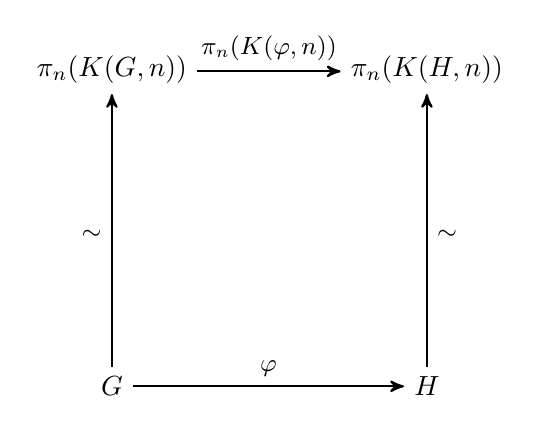
\begin{tikzpicture}[>=stealth',auto,node distance=3cm,
      thick,main node/.style={font=\sffamily\bfseries},text height=1.5ex]
    \node[main node] (KG) at (0,0) {$\pi_n(K(G,n))$};
    \node[main node] (KH) at (4,0) {$\pi_n(K(H,n))$};
    \node[main node] (G) at (0,-4) {$G$};
    \node[main node] (H) at (4,-4) {$H$};
         \path[every node/.style={font=\sffamily\small}]
         (KG) edge [->] node {$\pi_n(K(\phi,n))$} (KH)
         (G)  edge [->] node [left] {$\sim$} (KG)
              edge [->] node {$\phi$} (H)
         (H)  edge [->] node [right] {$\sim$} (KH);
  \end{tikzpicture}
\end{center}

\end{lemma}
\begin{proof}
\end{proof}

\begin{lemma}
The following diagram commutes.
\begin{center}
  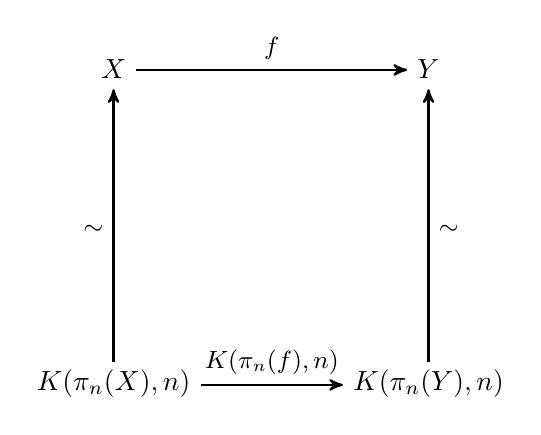
\begin{tikzpicture}[>=stealth',auto,node distance=3cm,
      thick,main node/.style={font=\sffamily\bfseries},text height=1.5ex]
    \node[main node] (X)  at (0,0) {$X$};
    \node[main node] (Y)  at (4,0) {$Y$};
    \node[main node] (KX) at (0,-4) {$K(\pi_n(X),n)$};
    \node[main node] (KY) at (4,-4) {$K(\pi_n(Y),n)$};
         \path[every node/.style={font=\sffamily\small}]
         (X)  edge [->] node {$f$} (Y)
         (KX) edge [->] node [left] {$\sim$} (X)
              edge [->] node {$K(\pi_n(f),n)$} (KY)
         (KY) edge [->] node [right] {$\sim$} (Y);
  \end{tikzpicture}
\end{center}

\end{lemma}
\begin{proof}
\end{proof}

\begin{theorem}
  $K({-},n)$ is an equivalence from the category of $(n-1)$-connected $n$-truncated pointed types to
  the category of groups (for $n=1$) or Abelian groups (for $n\geq2$).
\end{theorem}
\begin{proof}
\end{proof}
\bibliographystyle{alpha}
{\footnotesize \bibliography{references}}

%% \bibliography{proptrunc}


\end{document}
